
\chapter{Computing Performance of sequential code\label{chpt:seq-code-performance}}

This section evaluates the computing performance of the code. Our
goal is to show that the new algorithm of angular convolution is faster
than the old naive one, and the huge amount of simulation has shown
that is absolutely the case. But a raw result, where the implementation
goes for an indefinite number of iterations during minimization, cannot %'evolution' or 'evaluation'?
give a proper and systematic performance evolution. That is the 
purpose of this section. 

As discussed in appendix \ref{chpt:computing-performance}, two main
factors influence the performance of a sequential code: the
algorithm complexity, and the memory delay. To study the algorithm
complexity, testing with respect to parameters is done on some simple
but important components. The result can match the theoretical algorithm
complexity, or be completely different due to the overhead of function
calling or the inhomogeneity of memory access. Study of these small %Slipped in a bit of French, I see.
parts permits a further understanding of the entire code.

\section{FFT}

The \acs{FFT} play an important role in the implementation, which
is used by the spatial convolution and the \acs{FGSHT} process. 

\begin{figure}[H]
\begin{centering}
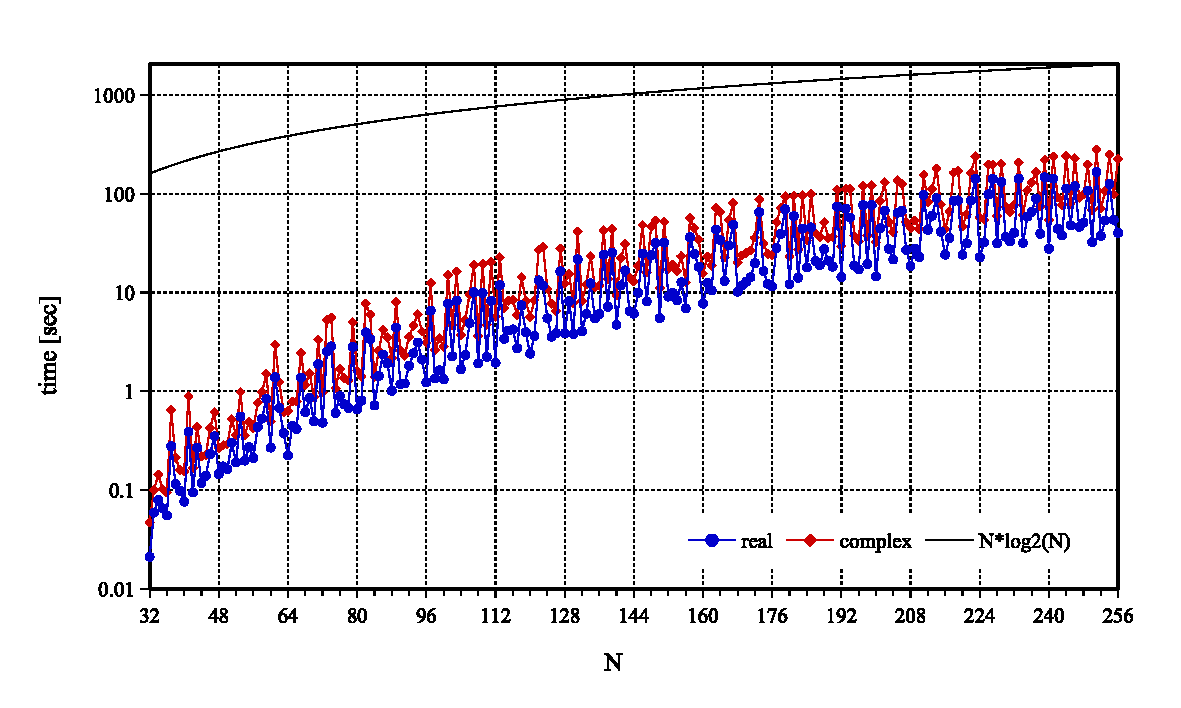
\includegraphics[bb=0bp 20bp 567bp 310bp,width=1\columnwidth]{_figure/results/fftw_timing}
\par\end{centering}
\caption{timing FFT\label{fig:timing-FFT}}
\end{figure}

Referring to figure \ref{fig:timing-FFT}, the dependance on $O(N\log_{2}N)$
\textcolor{red}{\scriptsize{}\citep{Numerical_Recipes_3ed}} doesn't
totally exist, but of the same form, depending on the algorithm of FFT
{[}ref dft{]}. It should be noted that a grid of prime number is always
at the peaks in the figure, which means il can be 2 or more time longer
than that of the composite number around. That means we should use
a even number grid, where the $k$-border correction in $\mathsection$\ref{subsec:k-border-effect}
is absolutely needed. Apart from this conclusion, to compare between
the algorithms for angular part involved in this thesis, we are not
really interested in computing performance with respect to the number
of spatial grid. However, the ratio of real and complex FFT timing
is important, as shown in figure \ref{fig:fft-real-to-complex}, which
is near the theoretical ratio 0.5. For example, we process $n_{\mathrm{angle}}$
real to complex FFT, then $n_{\mathrm{spatial}}/2$ complex to complex
FGSHT, or we process $n_{\mathrm{spatial}}$ real to complex FGSHT,
then $n_{\mathrm{proj}}/2$ complex to complex FFT, should not give
a great difference if $n_{\mathrm{angle}}\sim n_{\mathrm{proj}}$
for small $n_{\max}$. If it is not the case, it will have an influence
to the choice of algorithm.
\begin{center}
\begin{figure}[h]
\begin{centering}
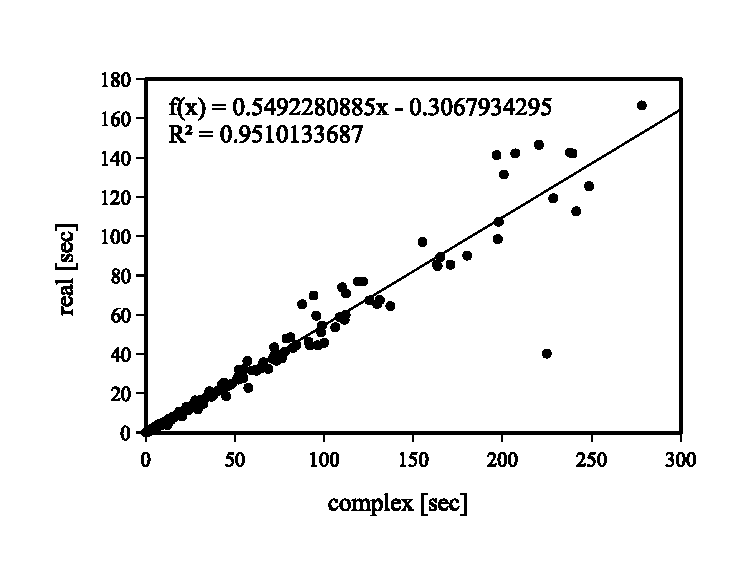
\includegraphics[bb=0bp 20bp 340bp 235bp,width=0.5\columnwidth]{_figure/results/fftw_real_v_cmplx}
\par\end{centering}
\caption{FFT real to complex\label{fig:fft-real-to-complex}}
\end{figure}
\par\end{center}

\section{FGSHT}

The computing times of GSHT and FGSHT are shown in figure \ref{fig:time-gsht-fgsht}.
There is no interest to see in detail how much FFT have accelerate
the GSHT process, but clearly FGSHT can be 100 times faster than GSHT,
and GSHT for the symmetry of $\Psi$, $s=1$ is in average 5 times
longer than $s=2$. As accuracy test shows that GSHT and FGSHT gives
exactly the same result, it is free to utilize FGSHT in all the case
to have a faster performance.
\begin{center}
\begin{figure}[H]
\begin{centering}
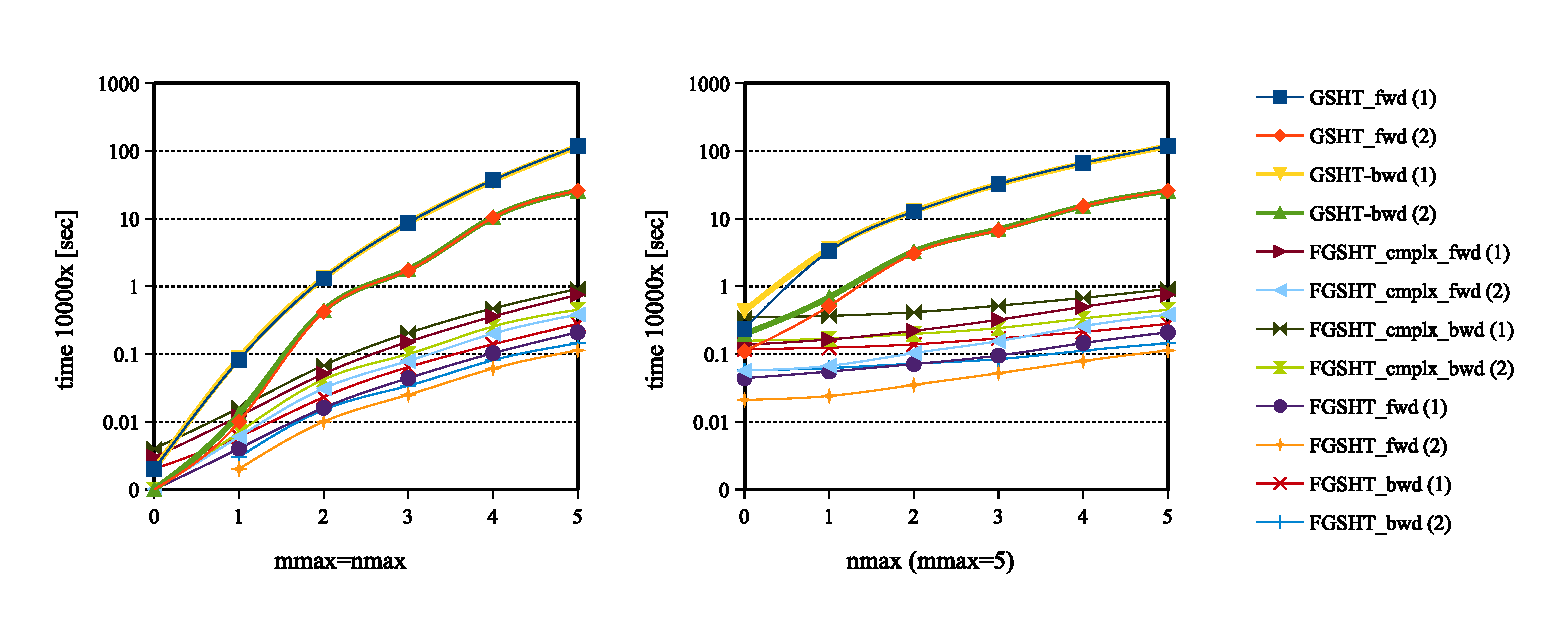
\includegraphics[bb=0bp 20bp 731bp 263bp,width=1\columnwidth]{_figure/results/fgsht_perf}
\par\end{centering}
\caption{Computing time of GSHT and FGSHT (per 10000 times), between parentheses
is the order of symmetry axes $s$\label{fig:time-gsht-fgsht}}
\end{figure}
\par\end{center}

However, it is important to know the ratio between real and complex
FGSHT process for the same reason as FFT. it is shown that this number
is 0.3 in all cases, and it does not depend on $n_{\max}$. The difference
between these two is that the real one performs real-to-complex FFT
for the $\Phi,\Psi$ grid and calculate only a half plus a bit of
projections ($\mu\geq0$) than the complex one. Normally, the ratio
should be greater than 0.5. This means there maybe an extra process
in the complex one or it is controlled by the memory. In a word, the
final result 0.3 means, that doing $n_{\mathrm{spatial}}$ real to
complex FGSHT takes only 0.6 times of doing $n_{\mathrm{spatial}}/2$
complex to complex FGSHT, which means in \texttt{\textbf{convolution\_standard}}
we use less time to compute FGSHT than in \texttt{\textbf{convolution\_pure\_angular}}.
\begin{center}
\begin{figure}[H]
\begin{centering}
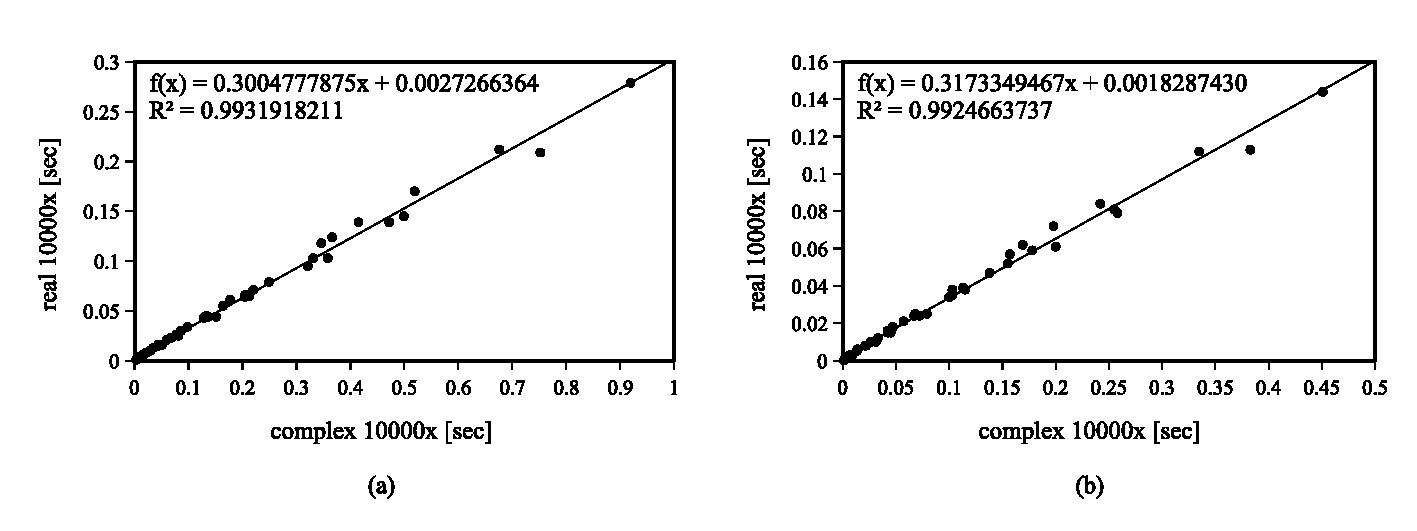
\includegraphics[bb=0bp 20bp 680bp 235bp,width=1\columnwidth]{_figure/results/fgsht_real_v_cmplx}
\par\end{centering}
\caption{FGSHT real to complex\label{fig:fgsht-real-to-complex}}
\end{figure}
\par\end{center}

\section{$k$-kernel}

As discussed in the previous section, the final result of energy and
structure is independent to the choice of path inside a $k$-kernel.
That means, it is free in precision cost to choose the fast path.
As path (1) and (2) in figure \ref{fig:k-kernel}introduce the transform
from $\Delta\hat{\rho}_{\mu'\mu}^{m}(\mathbf{k})$ to $\Delta\hat{\rho}(\mathbf{k},\mathbf{\Omega})$
that has no interest in timing, and the entire branches will be compared
in later implementation, here we only compare the path (3) and (4),
which correspond to eq. (\ref{eq:im}) and (\ref{eq:gamma-blum}).

The theoretical predictions of the computing time of \acs{OZ} equation
with respect to $n_{\max}$ are listed in table \ref{tab:FE-of-OZ}.
If the \acs{OZ} equation is the most time demanding part, the result
should have the same proposal. figure \ref{fig:k-kernel} shows the
experimental timing of the whole path (3) and (4).

It is shown that... \textcolor{red}{(There is a problem of code that
gives backtrace but obviously (4) is 100 times faster than (3).)}

\section{Entire iteration of $\mathcal{F}_{\mathrm{exc}}$ evaluation}

Apart from all the \texttt{\textbf{naive}} methods that will be discussed
in $\mathsection$\ref{subsec:Comparison-between-naive_standar},
figure \ref{fig:Entire-iteration} shows all the comparable \texttt{\textbf{convolution}}
timing data. We can see \texttt{\textbf{convolution\_standard}} is
the fastest algorithm, and OZ equation is not the longest part in
the iteration. All the tests are performed for a $L=24$, $\mathrm{nfft}=72$
grid, with 4 series: the three \texttt{\textbf{convolution}} methods
with$m_{\max}=n_{\max}$, and \texttt{\textbf{convolution\_standard}}
with $m_{\max}=5$, varying $n_{\max}$.

\begin{figure}[H]
\begin{centering}
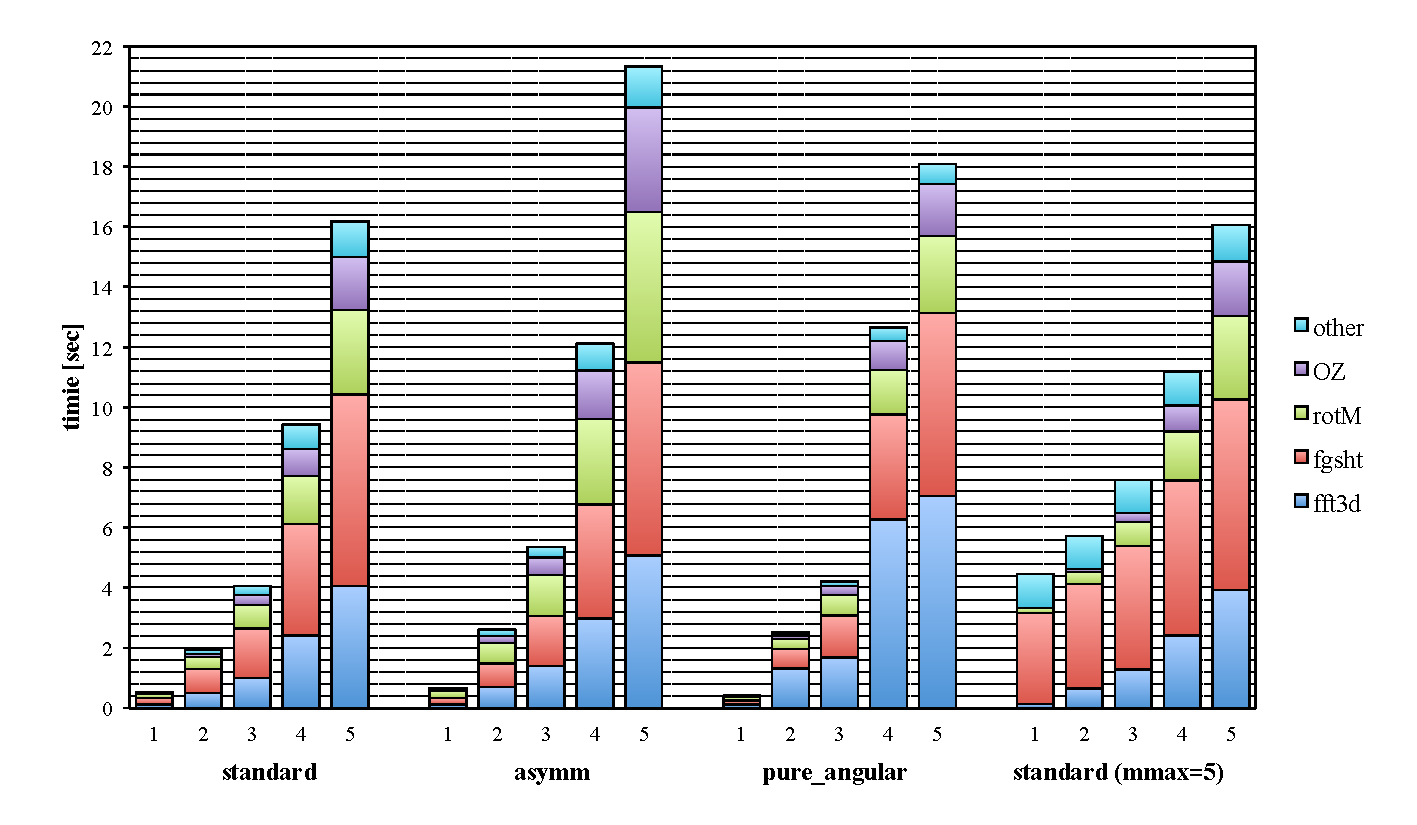
\includegraphics[bb=0cm 1cm 24cm 13cm,width=0.9\columnwidth]{_figure/results/branch_perf}
\par\end{centering}
\caption{Entire iteration of $\mathcal{F}_{\mathrm{exc}}$ evaluation: timing
overall \label{fig:Entire-iteration}}
\end{figure}


\subsection{Comparison between ``naive'' methods and ``convolution\_pure\_angular''\label{subsec:Comparison-between-naive_standar}}

The \texttt{\textbf{naive\_standard}}, \texttt{\textbf{naive\_interpolation}},
and \texttt{\textbf{convolution\_pure\_angular}} methods share the
same processes out of the $k$-kernel. Table \ref{tab:Timing-loop-k}
shows the timing of loop $k$ of these three methods. It is shown
that \texttt{\textbf{convolution\_pure\_angular}} takes far less time
than other two methods, of which the loop $k$ takes time in the same
order of magnitude than the rest of iteration. And once $m_{\max}\geq2$,
\texttt{\textbf{naive\_interpolation}} is faster than \texttt{\textbf{naive\_standard}}.
Note that order 2 of \texttt{\textbf{naive\_interpolation}} can give
already good result for a DCF of $n_{\max}=5$. So in every case of
\texttt{\textbf{naive}} methods, \texttt{\textbf{naive\_interpolation}}
should be used. This verified the conclusion of $k$-kernel test,
that the path (4) in figure \ref{fig:k-kernel} is the fastest.

\begin{table}[H]
\begin{centering}
\begin{tabular}{lllll}
\toprule 
$m_{\max}$ & \texttt{\textbf{naive\_standard}} & \texttt{\textbf{naive\_interpolation}} & \texttt{\textbf{convo\_pure\_angular}} & \tableheadline{Other}\tabularnewline
\midrule
1 & 2.34 & 4.42 & 0.26 & 0.15\tabularnewline
2 & 365.95 & 209.12 & 1.09 & 1.43\tabularnewline
3 & 3295.00 & 752.70 & 2.37 & 1.85\tabularnewline
\bottomrule
\end{tabular}
\par\end{centering}
\caption{Timing {[}sec{]} of loop $k$ of ``naive\_standard'', ``naive\_interpolation''
and ``convolution\_pure\_angular'', and the rest of iteration\label{tab:Timing-loop-k}}
\end{table}


\subsection{Comparison ``convolution\_standard'' and ``convolution\_pure\_angular''}

The comparison of \texttt{\textbf{convolution\_standard}} and \texttt{\textbf{convolution\_pure\_angular}}
is shown in figure \ref{fig:comparison-pure_angular}. Their difference
is the inversion of FFT and FGSHT. We can see the other parts are
almost identical, but the implementation of FFT takes different time.
Because in \texttt{\textbf{convolution\_standard}} the number of FE
we need for FFT is the number of projections, and in \texttt{\textbf{convolution\_pure\_angular}}
it is the number of angular grid nodes. As there is less projections
than angular nodes, \texttt{\textbf{convolution\_standard}} reasonably
takes less time.

\begin{figure}[H]
\begin{centering}
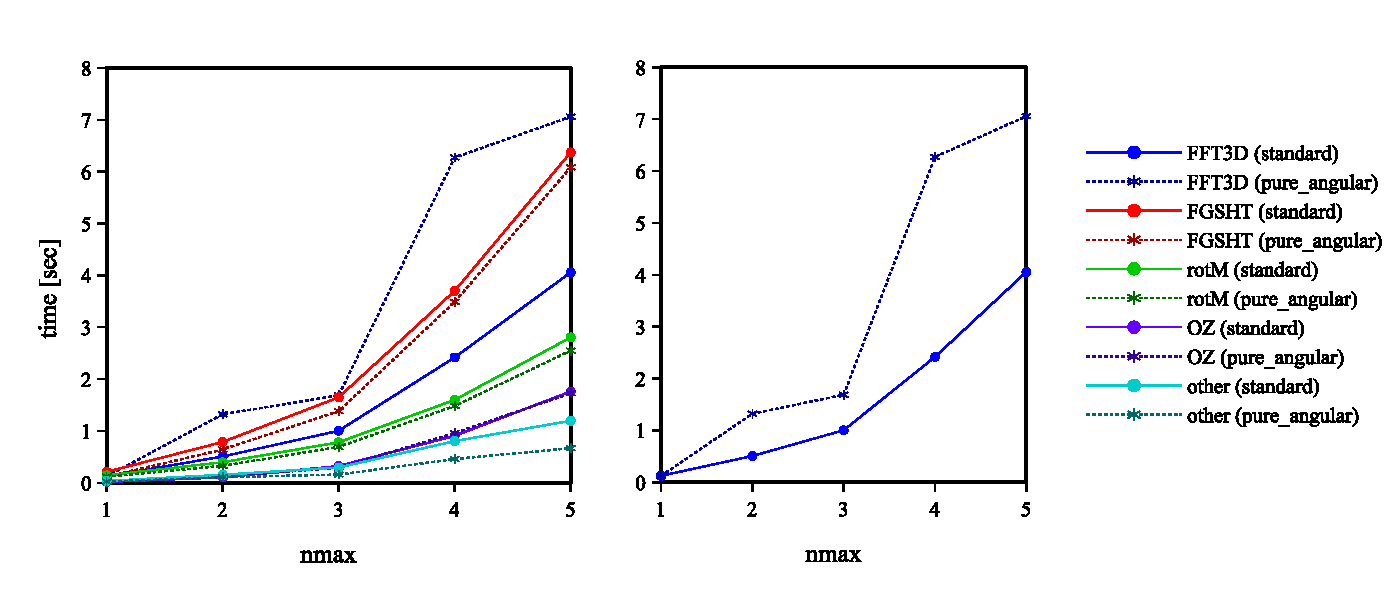
\includegraphics[bb=0bp 20bp 432bp 268bp,scale=0.6]{_figure/results/pure_angular}
\par\end{centering}
\caption{comparison of \texttt{\textbf{convolution\_standard}} and \texttt{\textbf{convolution\_pure\_angular\label{fig:comparison-pure_angular}}}}
\end{figure}


\subsection{Comparison ``convolution\_standard'' and ``convolution\_asymm''}

The comparison of \texttt{\textbf{convolution\_standard}} and \texttt{\textbf{convolution\_asymm}}
is shown in figure \ref{fig:comparison-asymm}. Their difference is
that \texttt{\textbf{standard}} calculate a half $k$ in the $k$loop
and \texttt{\textbf{asymm}} calculate all $k$ in the $k$loop. They
share the same process of FGSHT; for the processes in a $k$ loop
(rotM, OZ) \texttt{\textbf{asymm}} takes always longer time. As in
\texttt{\textbf{asymm}} we calculate the FFT for all the projections;
and in \texttt{\textbf{standard}} we calculate only a half projections
with $\mu\geq0$, it is also different.

\begin{figure}[H]
\begin{centering}
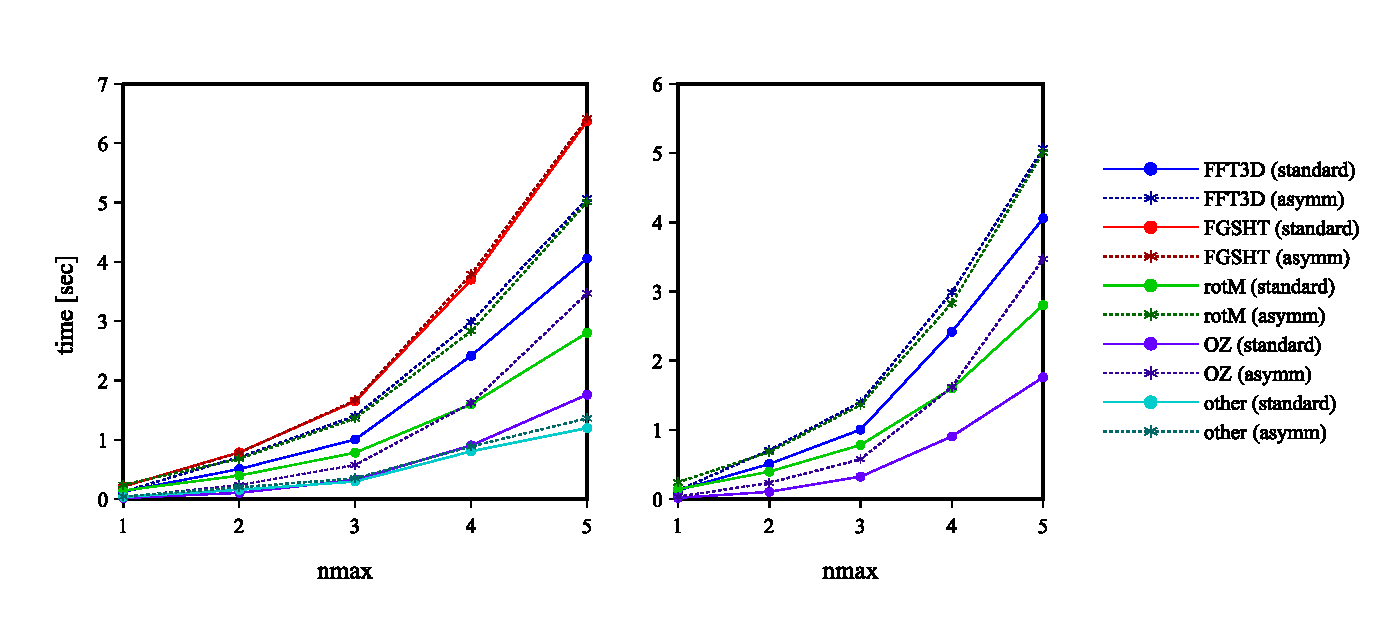
\includegraphics[bb=0bp 20bp 432bp 268bp,scale=0.6]{_figure/results/asymm}
\par\end{centering}
\caption{comparison of \texttt{\textbf{convolution\_standard}} and \texttt{\textbf{convolution\_asymm\label{fig:comparison-asymm}}}}
\end{figure}


\subsection{Comparison mmax and nmax}

The comparison of $m_{\max}=n_{\max}$ and $m_{\max}=5$ for\texttt{\textbf{
convolution\_standard}} is shown in figure \ref{fig:comparison-nmax}.
We see that the choice of quadrature order $m_{\max}$ only affect
the FGSHT process and the lecture/storage of density variable (other).

\begin{figure}[H]
\begin{centering}
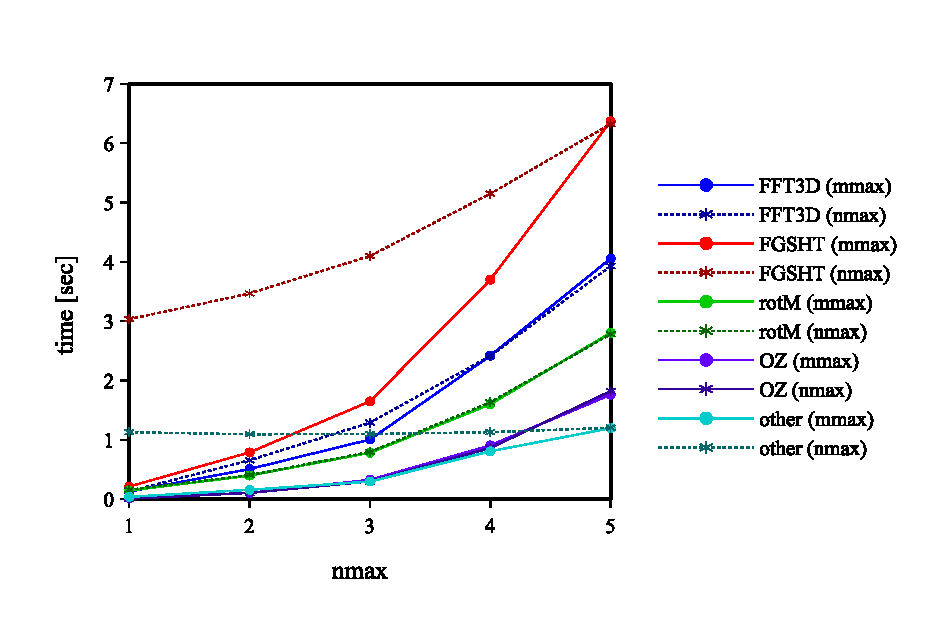
\includegraphics[bb=0bp 20bp 432bp 268bp,scale=0.6]{_figure/results/nmax}
\par\end{centering}
\caption{comparison of \texttt{\textbf{convolution\_standard}} for $m_{\max}=n_{\max}$
and $m_{\max}=5$\label{fig:comparison-nmax}}
\end{figure}


\section{Global view of the sequential code performance}

We can see that \texttt{\textbf{convolution\_standard}} is the fastest.
The \texttt{\textbf{convolution}} methods are of magnitude faster
than \texttt{\textbf{naive}} methods.
